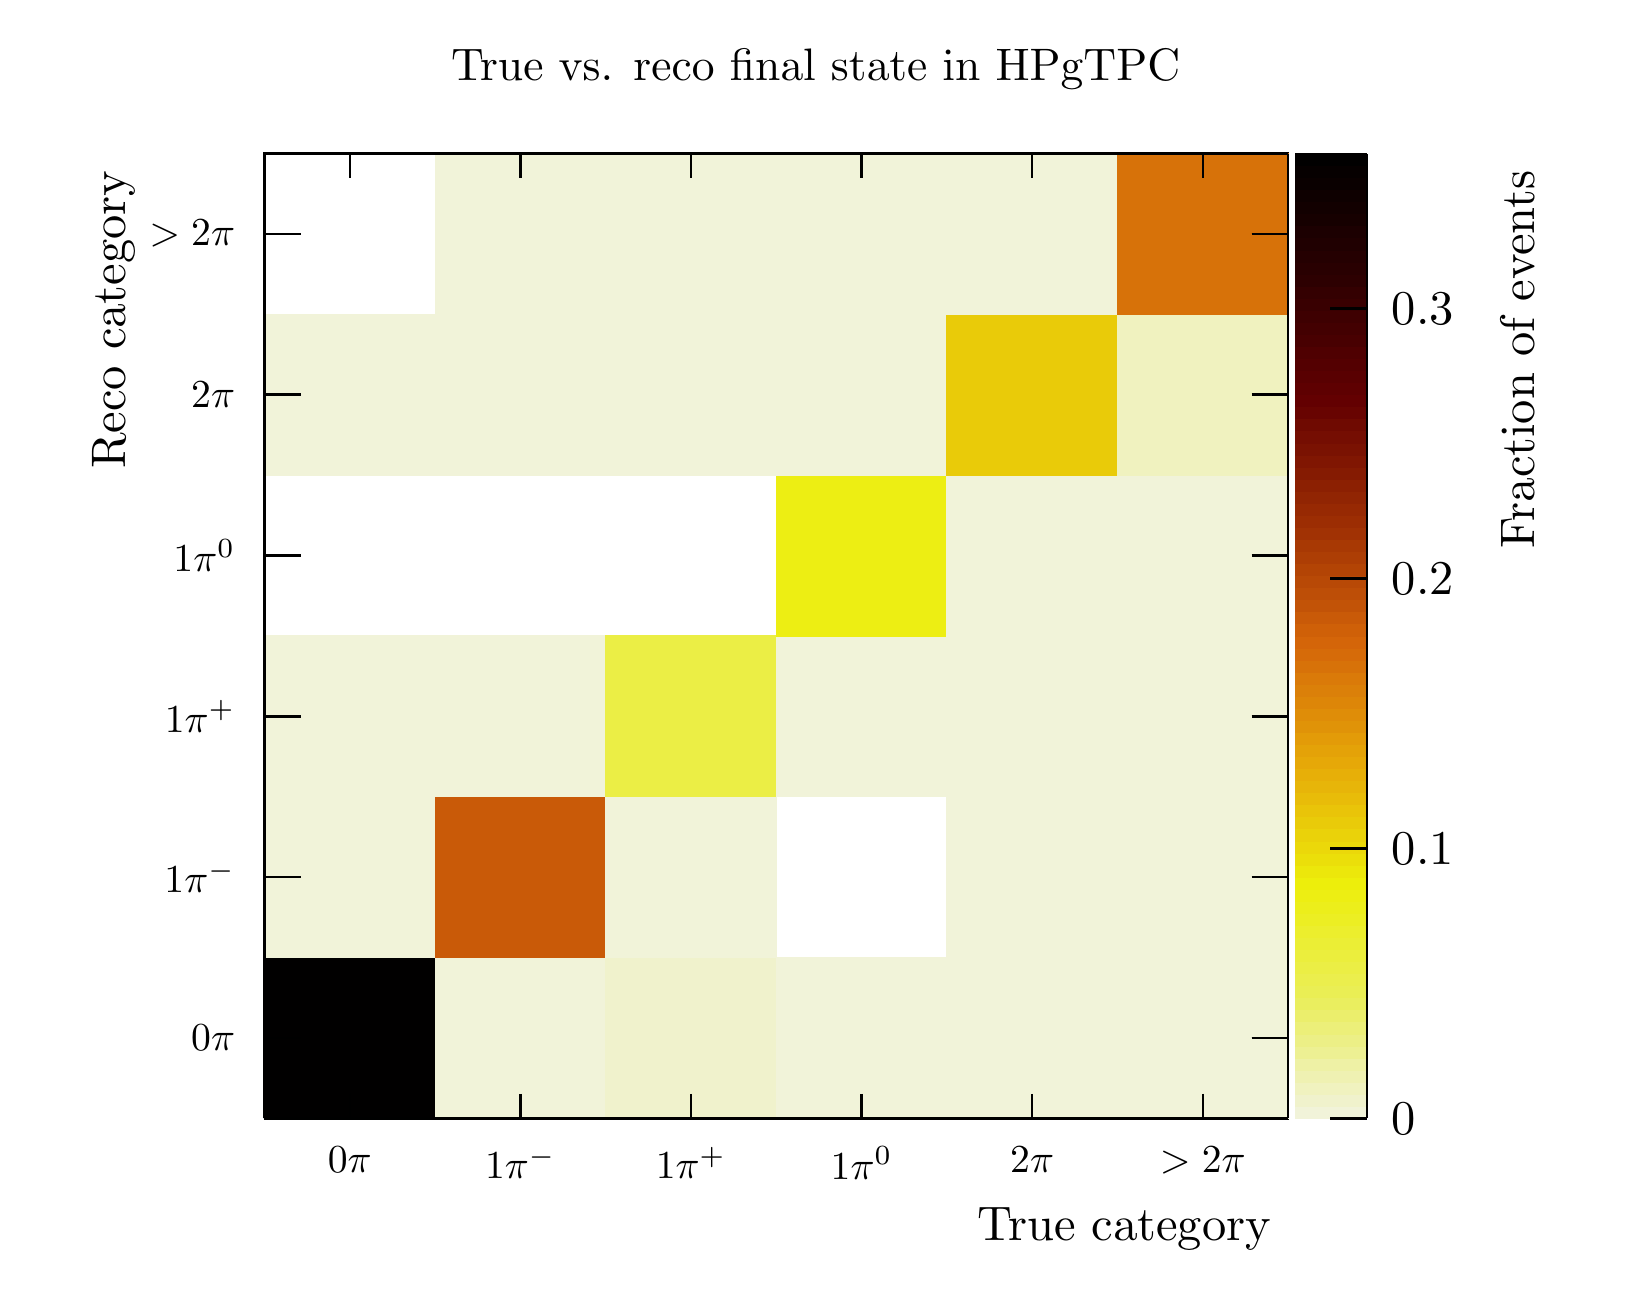
\begin{tikzpicture}
\pgfdeclareplotmark{cross} {
\pgfpathmoveto{\pgfpoint{-0.3\pgfplotmarksize}{\pgfplotmarksize}}
\pgfpathlineto{\pgfpoint{+0.3\pgfplotmarksize}{\pgfplotmarksize}}
\pgfpathlineto{\pgfpoint{+0.3\pgfplotmarksize}{0.3\pgfplotmarksize}}
\pgfpathlineto{\pgfpoint{+1\pgfplotmarksize}{0.3\pgfplotmarksize}}
\pgfpathlineto{\pgfpoint{+1\pgfplotmarksize}{-0.3\pgfplotmarksize}}
\pgfpathlineto{\pgfpoint{+0.3\pgfplotmarksize}{-0.3\pgfplotmarksize}}
\pgfpathlineto{\pgfpoint{+0.3\pgfplotmarksize}{-1.\pgfplotmarksize}}
\pgfpathlineto{\pgfpoint{-0.3\pgfplotmarksize}{-1.\pgfplotmarksize}}
\pgfpathlineto{\pgfpoint{-0.3\pgfplotmarksize}{-0.3\pgfplotmarksize}}
\pgfpathlineto{\pgfpoint{-1.\pgfplotmarksize}{-0.3\pgfplotmarksize}}
\pgfpathlineto{\pgfpoint{-1.\pgfplotmarksize}{0.3\pgfplotmarksize}}
\pgfpathlineto{\pgfpoint{-0.3\pgfplotmarksize}{0.3\pgfplotmarksize}}
\pgfpathclose
\pgfusepathqstroke
}
\pgfdeclareplotmark{cross*} {
\pgfpathmoveto{\pgfpoint{-0.3\pgfplotmarksize}{\pgfplotmarksize}}
\pgfpathlineto{\pgfpoint{+0.3\pgfplotmarksize}{\pgfplotmarksize}}
\pgfpathlineto{\pgfpoint{+0.3\pgfplotmarksize}{0.3\pgfplotmarksize}}
\pgfpathlineto{\pgfpoint{+1\pgfplotmarksize}{0.3\pgfplotmarksize}}
\pgfpathlineto{\pgfpoint{+1\pgfplotmarksize}{-0.3\pgfplotmarksize}}
\pgfpathlineto{\pgfpoint{+0.3\pgfplotmarksize}{-0.3\pgfplotmarksize}}
\pgfpathlineto{\pgfpoint{+0.3\pgfplotmarksize}{-1.\pgfplotmarksize}}
\pgfpathlineto{\pgfpoint{-0.3\pgfplotmarksize}{-1.\pgfplotmarksize}}
\pgfpathlineto{\pgfpoint{-0.3\pgfplotmarksize}{-0.3\pgfplotmarksize}}
\pgfpathlineto{\pgfpoint{-1.\pgfplotmarksize}{-0.3\pgfplotmarksize}}
\pgfpathlineto{\pgfpoint{-1.\pgfplotmarksize}{0.3\pgfplotmarksize}}
\pgfpathlineto{\pgfpoint{-0.3\pgfplotmarksize}{0.3\pgfplotmarksize}}
\pgfpathclose
\pgfusepathqfillstroke
}
\pgfdeclareplotmark{newstar} {
\pgfpathmoveto{\pgfqpoint{0pt}{\pgfplotmarksize}}
\pgfpathlineto{\pgfqpointpolar{44}{0.5\pgfplotmarksize}}
\pgfpathlineto{\pgfqpointpolar{18}{\pgfplotmarksize}}
\pgfpathlineto{\pgfqpointpolar{-20}{0.5\pgfplotmarksize}}
\pgfpathlineto{\pgfqpointpolar{-54}{\pgfplotmarksize}}
\pgfpathlineto{\pgfqpointpolar{-90}{0.5\pgfplotmarksize}}
\pgfpathlineto{\pgfqpointpolar{234}{\pgfplotmarksize}}
\pgfpathlineto{\pgfqpointpolar{198}{0.5\pgfplotmarksize}}
\pgfpathlineto{\pgfqpointpolar{162}{\pgfplotmarksize}}
\pgfpathlineto{\pgfqpointpolar{134}{0.5\pgfplotmarksize}}
\pgfpathclose
\pgfusepathqstroke
}
\pgfdeclareplotmark{newstar*} {
\pgfpathmoveto{\pgfqpoint{0pt}{\pgfplotmarksize}}
\pgfpathlineto{\pgfqpointpolar{44}{0.5\pgfplotmarksize}}
\pgfpathlineto{\pgfqpointpolar{18}{\pgfplotmarksize}}
\pgfpathlineto{\pgfqpointpolar{-20}{0.5\pgfplotmarksize}}
\pgfpathlineto{\pgfqpointpolar{-54}{\pgfplotmarksize}}
\pgfpathlineto{\pgfqpointpolar{-90}{0.5\pgfplotmarksize}}
\pgfpathlineto{\pgfqpointpolar{234}{\pgfplotmarksize}}
\pgfpathlineto{\pgfqpointpolar{198}{0.5\pgfplotmarksize}}
\pgfpathlineto{\pgfqpointpolar{162}{\pgfplotmarksize}}
\pgfpathlineto{\pgfqpointpolar{134}{0.5\pgfplotmarksize}}
\pgfpathclose
\pgfusepathqfillstroke
}
\definecolor{c}{rgb}{1,1,1};
\draw [color=c, fill=c] (0,0) rectangle (20,15.914);
\draw [color=c, fill=c] (3,2.06882) rectangle (16,14.3226);
\definecolor{c}{rgb}{0,0,0};
\draw [c,line width=0.9] (3,2.06882) -- (3,14.3226) -- (16,14.3226) -- (16,2.06882) -- (3,2.06882);
\definecolor{c}{rgb}{1,1,1};
\draw [color=c, fill=c] (3,2.06882) rectangle (16,14.3226);
\definecolor{c}{rgb}{0,0,0};
\draw [c,line width=0.9] (3,2.06882) -- (3,14.3226) -- (16,14.3226) -- (16,2.06882) -- (3,2.06882);
\definecolor{c}{rgb}{0.00551471,0,0.000122549};
\draw [color=c, fill=c] (3,2.06882) rectangle (5.16667,4.11111);
\definecolor{c}{rgb}{0.945984,0.951044,0.850727};
\draw [color=c, fill=c] (5.16667,2.06882) rectangle (7.33333,4.11111);
\definecolor{c}{rgb}{0.942948,0.949146,0.799494};
\draw [color=c, fill=c] (7.33333,2.06882) rectangle (9.5,4.11111);
\definecolor{c}{rgb}{0.945984,0.951044,0.850727};
\draw [color=c, fill=c] (9.5,2.06882) rectangle (11.6667,4.11111);
\draw [color=c, fill=c] (11.6667,2.06882) rectangle (13.8333,4.11111);
\draw [color=c, fill=c] (13.8333,2.06882) rectangle (16,4.11111);
\draw [color=c, fill=c] (3,4.11111) rectangle (5.16667,6.15341);
\definecolor{c}{rgb}{0.790196,0.354902,0.0308824};
\draw [color=c, fill=c] (5.16667,4.11111) rectangle (7.33333,6.15341);
\definecolor{c}{rgb}{0.945984,0.951044,0.850727};
\draw [color=c, fill=c] (7.33333,4.11111) rectangle (9.5,6.15341);
\draw [color=c, fill=c] (11.6667,4.11111) rectangle (13.8333,6.15341);
\draw [color=c, fill=c] (13.8333,4.11111) rectangle (16,6.15341);
\draw [color=c, fill=c] (3,6.15341) rectangle (5.16667,8.1957);
\draw [color=c, fill=c] (5.16667,6.15341) rectangle (7.33333,8.1957);
\definecolor{c}{rgb}{0.921324,0.933333,0.269608};
\draw [color=c, fill=c] (7.33333,6.15341) rectangle (9.5,8.1957);
\definecolor{c}{rgb}{0.945984,0.951044,0.850727};
\draw [color=c, fill=c] (9.5,6.15341) rectangle (11.6667,8.1957);
\draw [color=c, fill=c] (11.6667,6.15341) rectangle (13.8333,8.1957);
\draw [color=c, fill=c] (13.8333,6.15341) rectangle (16,8.1957);
\definecolor{c}{rgb}{0.928309,0.933333,0.0740196};
\draw [color=c, fill=c] (9.5,8.1957) rectangle (11.6667,10.238);
\definecolor{c}{rgb}{0.945984,0.951044,0.850727};
\draw [color=c, fill=c] (11.6667,8.1957) rectangle (13.8333,10.238);
\draw [color=c, fill=c] (13.8333,8.1957) rectangle (16,10.238);
\draw [color=c, fill=c] (3,10.238) rectangle (5.16667,12.2803);
\draw [color=c, fill=c] (5.16667,10.238) rectangle (7.33333,12.2803);
\draw [color=c, fill=c] (7.33333,10.238) rectangle (9.5,12.2803);
\draw [color=c, fill=c] (9.5,10.238) rectangle (11.6667,12.2803);
\definecolor{c}{rgb}{0.915686,0.796078,0.0372549};
\draw [color=c, fill=c] (11.6667,10.238) rectangle (13.8333,12.2803);
\definecolor{c}{rgb}{0.939911,0.947249,0.748261};
\draw [color=c, fill=c] (13.8333,10.238) rectangle (16,12.2803);
\definecolor{c}{rgb}{0.945984,0.951044,0.850727};
\draw [color=c, fill=c] (5.16667,12.2803) rectangle (7.33333,14.3226);
\draw [color=c, fill=c] (7.33333,12.2803) rectangle (9.5,14.3226);
\draw [color=c, fill=c] (9.5,12.2803) rectangle (11.6667,14.3226);
\draw [color=c, fill=c] (11.6667,12.2803) rectangle (13.8333,14.3226);
\definecolor{c}{rgb}{0.844608,0.445343,0.0345588};
\draw [color=c, fill=c] (13.8333,12.2803) rectangle (16,14.3226);
\definecolor{c}{rgb}{0,0,0};
\draw [c,line width=0.9] (3,2.06882) -- (16,2.06882);
\draw [anchor=north] (4.08333,1.88501) node[scale=1.43288, color=c, rotate=0]{$0\pi$};
\draw [anchor=north] (6.25,1.88501) node[scale=1.43288, color=c, rotate=0]{$1\pi^{-}$};
\draw [anchor=north] (8.41667,1.88501) node[scale=1.43288, color=c, rotate=0]{$1\pi^{+}$};
\draw [anchor=north] (10.5833,1.88501) node[scale=1.43288, color=c, rotate=0]{$1\pi^{0}$};
\draw [anchor=north] (12.75,1.88501) node[scale=1.43288, color=c, rotate=0]{$2\pi$};
\draw [anchor=north] (14.9167,1.88501) node[scale=1.43288, color=c, rotate=0]{$>2\pi$};
\draw [c,line width=0.9] (4.08333,2.37914) -- (4.08333,2.06882);
\draw [c,line width=0.9] (6.25,2.37914) -- (6.25,2.06882);
\draw [c,line width=0.9] (8.41667,2.37914) -- (8.41667,2.06882);
\draw [c,line width=0.9] (10.5833,2.37914) -- (10.5833,2.06882);
\draw [c,line width=0.9] (12.75,2.37914) -- (12.75,2.06882);
\draw [c,line width=0.9] (14.9167,2.37914) -- (14.9167,2.06882);
\draw [c,line width=0.9] (4.08333,2.37914) -- (4.08333,2.06882);
\draw [c,line width=0.9] (14.9167,2.37914) -- (14.9167,2.06882);
\draw [anchor= east] (16,0.668387) node[scale=1.7513, color=c, rotate=0]{ True category};
\draw [c,line width=0.9] (3,14.3226) -- (16,14.3226);
\draw [c,line width=0.9] (4.08333,14.0123) -- (4.08333,14.3226);
\draw [c,line width=0.9] (6.25,14.0123) -- (6.25,14.3226);
\draw [c,line width=0.9] (8.41667,14.0123) -- (8.41667,14.3226);
\draw [c,line width=0.9] (10.5833,14.0123) -- (10.5833,14.3226);
\draw [c,line width=0.9] (12.75,14.0123) -- (12.75,14.3226);
\draw [c,line width=0.9] (14.9167,14.0123) -- (14.9167,14.3226);
\draw [c,line width=0.9] (4.08333,14.0123) -- (4.08333,14.3226);
\draw [c,line width=0.9] (14.9167,14.0123) -- (14.9167,14.3226);
\draw [c,line width=0.9] (3,2.06882) -- (3,14.3226);
\draw [anchor= east] (2.805,3.08996) node[scale=1.43288, color=c, rotate=0]{$0\pi$};
\draw [anchor= east] (2.805,5.13226) node[scale=1.43288, color=c, rotate=0]{$1\pi^{-}$};
\draw [anchor= east] (2.805,7.17455) node[scale=1.43288, color=c, rotate=0]{$1\pi^{+}$};
\draw [anchor= east] (2.805,9.21685) node[scale=1.43288, color=c, rotate=0]{$1\pi^{0}$};
\draw [anchor= east] (2.805,11.2591) node[scale=1.43288, color=c, rotate=0]{$2\pi$};
\draw [anchor= east] (2.805,13.3014) node[scale=1.43288, color=c, rotate=0]{$>2\pi$};
\draw [c,line width=0.9] (3.462,3.08996) -- (3,3.08996);
\draw [c,line width=0.9] (3.462,5.13226) -- (3,5.13226);
\draw [c,line width=0.9] (3.462,7.17455) -- (3,7.17455);
\draw [c,line width=0.9] (3.462,9.21685) -- (3,9.21685);
\draw [c,line width=0.9] (3.462,11.2591) -- (3,11.2591);
\draw [c,line width=0.9] (3.462,13.3014) -- (3,13.3014);
\draw [c,line width=0.9] (3.462,3.08996) -- (3,3.08996);
\draw [c,line width=0.9] (3.462,13.3014) -- (3,13.3014);
\draw [anchor= east] (1.08,14.3226) node[scale=1.7513, color=c, rotate=90]{ Reco category};
\draw [c,line width=0.9] (16,2.06882) -- (16,14.3226);
\draw [c,line width=0.9] (15.538,3.08996) -- (16,3.08996);
\draw [c,line width=0.9] (15.538,5.13226) -- (16,5.13226);
\draw [c,line width=0.9] (15.538,7.17455) -- (16,7.17455);
\draw [c,line width=0.9] (15.538,9.21685) -- (16,9.21685);
\draw [c,line width=0.9] (15.538,11.2591) -- (16,11.2591);
\draw [c,line width=0.9] (15.538,13.3014) -- (16,13.3014);
\draw [c,line width=0.9] (15.538,3.08996) -- (16,3.08996);
\draw [c,line width=0.9] (15.538,13.3014) -- (16,13.3014);
\definecolor{c}{rgb}{0.945984,0.951044,0.850727};
\draw [color=c, fill=c] (16.1,2.06882) rectangle (17,2.22199);
\definecolor{c}{rgb}{0.942948,0.949146,0.799494};
\draw [color=c, fill=c] (16.1,2.22199) rectangle (17,2.37516);
\definecolor{c}{rgb}{0.939911,0.947249,0.748261};
\draw [color=c, fill=c] (16.1,2.37516) rectangle (17,2.52833);
\definecolor{c}{rgb}{0.936875,0.945351,0.697027};
\draw [color=c, fill=c] (16.1,2.52833) rectangle (17,2.68151);
\definecolor{c}{rgb}{0.933839,0.943453,0.645794};
\draw [color=c, fill=c] (16.1,2.68151) rectangle (17,2.83468);
\definecolor{c}{rgb}{0.929791,0.940923,0.577483};
\draw [color=c, fill=c] (16.1,2.83468) rectangle (17,2.98785);
\definecolor{c}{rgb}{0.926755,0.939026,0.526249};
\draw [color=c, fill=c] (16.1,2.98785) rectangle (17,3.14102);
\definecolor{c}{rgb}{0.923719,0.937128,0.475016};
\draw [color=c, fill=c] (16.1,3.14102) rectangle (17,3.29419);
\definecolor{c}{rgb}{0.920683,0.935231,0.423782};
\draw [color=c, fill=c] (16.1,3.29419) rectangle (17,3.44737);
\definecolor{c}{rgb}{0.917647,0.933333,0.372549};
\draw [color=c, fill=c] (16.1,3.44737) rectangle (17,3.60054);
\definecolor{c}{rgb}{0.919118,0.933333,0.331373};
\draw [color=c, fill=c] (16.1,3.60054) rectangle (17,3.75371);
\definecolor{c}{rgb}{0.920221,0.933333,0.30049};
\draw [color=c, fill=c] (16.1,3.75371) rectangle (17,3.90688);
\definecolor{c}{rgb}{0.921324,0.933333,0.269608};
\draw [color=c, fill=c] (16.1,3.90688) rectangle (17,4.06005);
\definecolor{c}{rgb}{0.922426,0.933333,0.238725};
\draw [color=c, fill=c] (16.1,4.06005) rectangle (17,4.21323);
\definecolor{c}{rgb}{0.923529,0.933333,0.207843};
\draw [color=c, fill=c] (16.1,4.21323) rectangle (17,4.3664);
\definecolor{c}{rgb}{0.924632,0.933333,0.176961};
\draw [color=c, fill=c] (16.1,4.3664) rectangle (17,4.51957);
\definecolor{c}{rgb}{0.926103,0.933333,0.135784};
\draw [color=c, fill=c] (16.1,4.51957) rectangle (17,4.67274);
\definecolor{c}{rgb}{0.927206,0.933333,0.104902};
\draw [color=c, fill=c] (16.1,4.67274) rectangle (17,4.82591);
\definecolor{c}{rgb}{0.928309,0.933333,0.0740196};
\draw [color=c, fill=c] (16.1,4.82591) rectangle (17,4.97909);
\definecolor{c}{rgb}{0.929412,0.933333,0.0431373};
\draw [color=c, fill=c] (16.1,4.97909) rectangle (17,5.13226);
\definecolor{c}{rgb}{0.926838,0.907598,0.0420343};
\draw [color=c, fill=c] (16.1,5.13226) rectangle (17,5.28543);
\definecolor{c}{rgb}{0.923407,0.873284,0.0405637};
\draw [color=c, fill=c] (16.1,5.28543) rectangle (17,5.4386);
\definecolor{c}{rgb}{0.920833,0.847549,0.0394608};
\draw [color=c, fill=c] (16.1,5.4386) rectangle (17,5.59177);
\definecolor{c}{rgb}{0.91826,0.821814,0.0383578};
\draw [color=c, fill=c] (16.1,5.59177) rectangle (17,5.74495);
\definecolor{c}{rgb}{0.915686,0.796078,0.0372549};
\draw [color=c, fill=c] (16.1,5.74495) rectangle (17,5.89812);
\definecolor{c}{rgb}{0.913113,0.770343,0.036152};
\draw [color=c, fill=c] (16.1,5.89812) rectangle (17,6.05129);
\definecolor{c}{rgb}{0.909681,0.736029,0.0346814};
\draw [color=c, fill=c] (16.1,6.05129) rectangle (17,6.20446);
\definecolor{c}{rgb}{0.907108,0.710294,0.0335784};
\draw [color=c, fill=c] (16.1,6.20446) rectangle (17,6.35763);
\definecolor{c}{rgb}{0.904534,0.684559,0.0324755};
\draw [color=c, fill=c] (16.1,6.35763) rectangle (17,6.51081);
\definecolor{c}{rgb}{0.901961,0.658824,0.0313726};
\draw [color=c, fill=c] (16.1,6.51081) rectangle (17,6.66398);
\definecolor{c}{rgb}{0.895343,0.634191,0.0317402};
\draw [color=c, fill=c] (16.1,6.66398) rectangle (17,6.81715);
\definecolor{c}{rgb}{0.888726,0.609559,0.0321078};
\draw [color=c, fill=c] (16.1,6.81715) rectangle (17,6.97032);
\definecolor{c}{rgb}{0.879902,0.576716,0.032598};
\draw [color=c, fill=c] (16.1,6.97032) rectangle (17,7.12349);
\definecolor{c}{rgb}{0.873284,0.552083,0.0329657};
\draw [color=c, fill=c] (16.1,7.12349) rectangle (17,7.27667);
\definecolor{c}{rgb}{0.866667,0.527451,0.0333333};
\draw [color=c, fill=c] (16.1,7.27667) rectangle (17,7.42984);
\definecolor{c}{rgb}{0.860049,0.502819,0.033701};
\draw [color=c, fill=c] (16.1,7.42984) rectangle (17,7.58301);
\definecolor{c}{rgb}{0.853431,0.478186,0.0340686};
\draw [color=c, fill=c] (16.1,7.58301) rectangle (17,7.73618);
\definecolor{c}{rgb}{0.844608,0.445343,0.0345588};
\draw [color=c, fill=c] (16.1,7.73618) rectangle (17,7.88935);
\definecolor{c}{rgb}{0.83799,0.420711,0.0349265};
\draw [color=c, fill=c] (16.1,7.88935) rectangle (17,8.04253);
\definecolor{c}{rgb}{0.831373,0.396078,0.0352941};
\draw [color=c, fill=c] (16.1,8.04253) rectangle (17,8.1957);
\definecolor{c}{rgb}{0.810784,0.37549,0.0330882};
\draw [color=c, fill=c] (16.1,8.1957) rectangle (17,8.34887);
\definecolor{c}{rgb}{0.790196,0.354902,0.0308824};
\draw [color=c, fill=c] (16.1,8.34887) rectangle (17,8.50204);
\definecolor{c}{rgb}{0.762745,0.327451,0.0279412};
\draw [color=c, fill=c] (16.1,8.50204) rectangle (17,8.65522);
\definecolor{c}{rgb}{0.742157,0.306863,0.0257353};
\draw [color=c, fill=c] (16.1,8.65522) rectangle (17,8.80839);
\definecolor{c}{rgb}{0.721569,0.286275,0.0235294};
\draw [color=c, fill=c] (16.1,8.80839) rectangle (17,8.96156);
\definecolor{c}{rgb}{0.70098,0.265686,0.0213235};
\draw [color=c, fill=c] (16.1,8.96156) rectangle (17,9.11473);
\definecolor{c}{rgb}{0.680392,0.245098,0.0191176};
\draw [color=c, fill=c] (16.1,9.11473) rectangle (17,9.2679);
\definecolor{c}{rgb}{0.659804,0.22451,0.0169118};
\draw [color=c, fill=c] (16.1,9.2679) rectangle (17,9.42107);
\definecolor{c}{rgb}{0.632353,0.197059,0.0139706};
\draw [color=c, fill=c] (16.1,9.42107) rectangle (17,9.57425);
\definecolor{c}{rgb}{0.611765,0.176471,0.0117647};
\draw [color=c, fill=c] (16.1,9.57425) rectangle (17,9.72742);
\definecolor{c}{rgb}{0.590809,0.159926,0.0110294};
\draw [color=c, fill=c] (16.1,9.72742) rectangle (17,9.88059);
\definecolor{c}{rgb}{0.569853,0.143382,0.0102941};
\draw [color=c, fill=c] (16.1,9.88059) rectangle (17,10.0338);
\definecolor{c}{rgb}{0.548897,0.126838,0.00955882};
\draw [color=c, fill=c] (16.1,10.0338) rectangle (17,10.1869);
\definecolor{c}{rgb}{0.520956,0.104779,0.00857843};
\draw [color=c, fill=c] (16.1,10.1869) rectangle (17,10.3401);
\definecolor{c}{rgb}{0.5,0.0882353,0.00784314};
\draw [color=c, fill=c] (16.1,10.3401) rectangle (17,10.4933);
\definecolor{c}{rgb}{0.479044,0.0716912,0.00710784};
\draw [color=c, fill=c] (16.1,10.4933) rectangle (17,10.6465);
\definecolor{c}{rgb}{0.458088,0.0551471,0.00637255};
\draw [color=c, fill=c] (16.1,10.6465) rectangle (17,10.7996);
\definecolor{c}{rgb}{0.437132,0.0386029,0.00563726};
\draw [color=c, fill=c] (16.1,10.7996) rectangle (17,10.9528);
\definecolor{c}{rgb}{0.409191,0.0165441,0.00465686};
\draw [color=c, fill=c] (16.1,10.9528) rectangle (17,11.106);
\definecolor{c}{rgb}{0.388235,0,0.00392157};
\draw [color=c, fill=c] (16.1,11.106) rectangle (17,11.2591);
\definecolor{c}{rgb}{0.368382,0,0.00392157};
\draw [color=c, fill=c] (16.1,11.2591) rectangle (17,11.4123);
\definecolor{c}{rgb}{0.348529,0,0.00392157};
\draw [color=c, fill=c] (16.1,11.4123) rectangle (17,11.5655);
\definecolor{c}{rgb}{0.328676,0,0.00392157};
\draw [color=c, fill=c] (16.1,11.5655) rectangle (17,11.7187);
\definecolor{c}{rgb}{0.308824,0,0.00392157};
\draw [color=c, fill=c] (16.1,11.7187) rectangle (17,11.8718);
\definecolor{c}{rgb}{0.282353,0,0.00392157};
\draw [color=c, fill=c] (16.1,11.8718) rectangle (17,12.025);
\definecolor{c}{rgb}{0.2625,0,0.00392157};
\draw [color=c, fill=c] (16.1,12.025) rectangle (17,12.1782);
\definecolor{c}{rgb}{0.242647,0,0.00392157};
\draw [color=c, fill=c] (16.1,12.1782) rectangle (17,12.3313);
\definecolor{c}{rgb}{0.222794,0,0.00392157};
\draw [color=c, fill=c] (16.1,12.3313) rectangle (17,12.4845);
\definecolor{c}{rgb}{0.202941,0,0.00392157};
\draw [color=c, fill=c] (16.1,12.4845) rectangle (17,12.6377);
\definecolor{c}{rgb}{0.176471,0,0.00392157};
\draw [color=c, fill=c] (16.1,12.6377) rectangle (17,12.7909);
\definecolor{c}{rgb}{0.159926,0,0.00355392};
\draw [color=c, fill=c] (16.1,12.7909) rectangle (17,12.944);
\definecolor{c}{rgb}{0.143382,0,0.00318627};
\draw [color=c, fill=c] (16.1,12.944) rectangle (17,13.0972);
\definecolor{c}{rgb}{0.126838,0,0.00281863};
\draw [color=c, fill=c] (16.1,13.0972) rectangle (17,13.2504);
\definecolor{c}{rgb}{0.110294,0,0.00245098};
\draw [color=c, fill=c] (16.1,13.2504) rectangle (17,13.4035);
\definecolor{c}{rgb}{0.0882353,0,0.00196078};
\draw [color=c, fill=c] (16.1,13.4035) rectangle (17,13.5567);
\definecolor{c}{rgb}{0.0716912,0,0.00159314};
\draw [color=c, fill=c] (16.1,13.5567) rectangle (17,13.7099);
\definecolor{c}{rgb}{0.0551471,0,0.00122549};
\draw [color=c, fill=c] (16.1,13.7099) rectangle (17,13.8631);
\definecolor{c}{rgb}{0.0386029,0,0.000857843};
\draw [color=c, fill=c] (16.1,13.8631) rectangle (17,14.0162);
\definecolor{c}{rgb}{0.0220588,0,0.000490196};
\draw [color=c, fill=c] (16.1,14.0162) rectangle (17,14.1694);
\definecolor{c}{rgb}{0.00551471,0,0.000122549};
\draw [color=c, fill=c] (16.1,14.1694) rectangle (17,14.3226);
\definecolor{c}{rgb}{0,0,0};
\draw [c,line width=0.9] (17,2.06882) -- (17,14.3226);
\draw [c,line width=0.9] (16.538,2.06882) -- (17,2.06882);
\draw [c,line width=0.9] (16.538,5.49645) -- (17,5.49645);
\draw [c,line width=0.9] (16.538,8.92408) -- (17,8.92408);
\draw [c,line width=0.9] (16.538,12.3517) -- (17,12.3517);
\draw [c,line width=0.9] (16.538,12.3517) -- (17,12.3517);
\draw [anchor= west] (17.1,2.06882) node[scale=1.7513, color=c, rotate=0]{0};
\draw [anchor= west] (17.1,5.49645) node[scale=1.7513, color=c, rotate=0]{0.1};
\draw [anchor= west] (17.1,8.92408) node[scale=1.7513, color=c, rotate=0]{0.2};
\draw [anchor= west] (17.1,12.3517) node[scale=1.7513, color=c, rotate=0]{0.3};
\draw [anchor= east] (18.92,14.3226) node[scale=1.7513, color=c, rotate=90]{ Fraction of events};
\definecolor{c}{rgb}{1,1,1};
\draw [color=c, fill=c] (2,14.9591) rectangle (18,15.8344);
\definecolor{c}{rgb}{0,0,0};
\draw (10,15.3968) node[scale=1.64516, color=c, rotate=0]{True vs. reco final state in HPgTPC};
\end{tikzpicture}
